\documentclass{article}

\usepackage[final]{pdfpages}
\setboolean{@twoside}{false}
\usepackage{hyperref}
\usepackage[toc,page]{appendix}
\usepackage{tikz}
\usepackage{graphicx}
\usepackage{caption}
\usepackage{subcaption}
\usepackage{amsmath}
\usepackage[letterpaper, top=1in, bottom=1in, left=1in, right=1in]{geometry}
\usepackage{listings}
\usepackage{color}
\definecolor{mygreen}{RGB}{28,172,0} % color values Red, Green, Blue
\definecolor{mylilas}{RGB}{170,55,241}
\lstset{language=Matlab,%
    basicstyle=\footnotesize,
    breaklines=true,%
    morekeywords={matlab2tikz},
    keywordstyle=\color{blue},%
    morekeywords=[2]{1}, keywordstyle=[2]{\color{black}},
    identifierstyle=\color{black},%
    stringstyle=\color{mylilas},
    commentstyle=\color{mygreen},%
    showstringspaces=false,%without this there will be a symbol in the places where there is a space
    numbers=left,%
    numberstyle={\tiny \color{black}},% size of the numbers
    numbersep=9pt, % this defines how far the numbers are from the text
    emph=[1]{for,end,break},emphstyle=[1]\color{red}, %some words to emphasise
    % emph=[2]{word1,word2}, emphstyle=[2]{style},
}

\title{ECSE 493 --- Controls\&Robotics Lab\\Lab 1 Report}
\author{\textbf{David Lavoie-Boutin} 260583602}

\date{\today}

\begin{document}

\maketitle
\section{}
\begin{itemize}
    \item [(a)] The equation of the DC motor given in the description is:
    $$J_m \ddot{\theta} + \left(b + \frac{K_tK_m}{R_a} \right)\dot{\theta} = \frac{K_t}{R_a} v_a$$

    Substituting the numbers provided in the equation above, we get:
    \begin{eqnarray}
    0.01 \ddot{\theta} + \left(0.001 + \frac{0.02 * 0.02}{10} \right)\dot{\theta} &=& \frac{0.02}{10} v_a\\
    0.01 \ddot{\theta} + 0.00104 \dot{\theta} &=&0.002 v_a
    \end{eqnarray}
    We then apply the Laplace Transform and get the following:
    \begin{eqnarray}
        &0.01 s^2 \Theta + 0.00104 s \Theta = 0.002 V\\
        &\frac{\Theta}{V} = \frac{1}{s}\frac{0.002}{0.01s + 0.00104}\\
        &\frac{\dot{\Theta}}{V} = \frac{0.002}{0.01s + 0.00104}
    \end{eqnarray}
\clearpage

    \item [(b)] Next we input this equation in Matlab to plot the steady-state response:
    \begin{lstlisting}[language=Matlab]
    num = 0.002;
    den = [0.01 0.00104];
    T = tf(num,den)
    step(T)
    \end{lstlisting}

    Which yields the plot in Figure~\ref{fig:stepa}

    \begin{figure}[!htb]
        \centering
        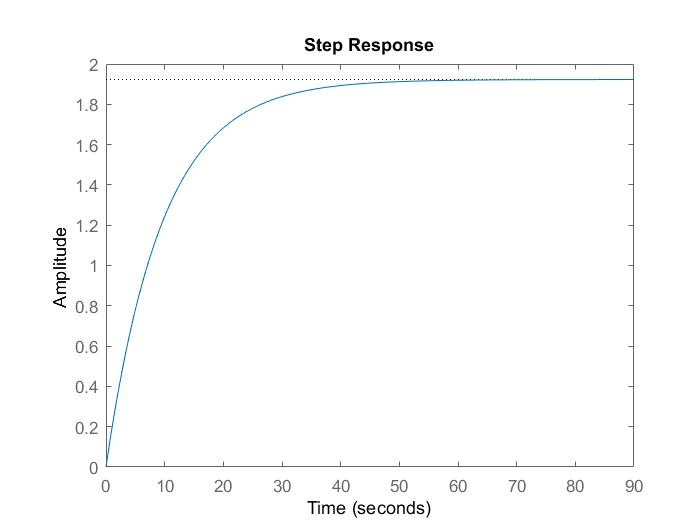
\includegraphics[width=.6\linewidth]{Step(a).jpg}
        \caption{Step response of motor shaft speed}
        \label{fig:stepa}
    \end{figure}
    With this plot, we can estimate the steady-state speed of the motor to be about 1.95 rad/sec.

    \item[(c)]
    If we assume our estimate in part (b), then 99\% of the final speed would be 1.88 rad/sec, which I estimate arrives at around 45 seconds
    \begin{figure}[!htb]
        \centering
        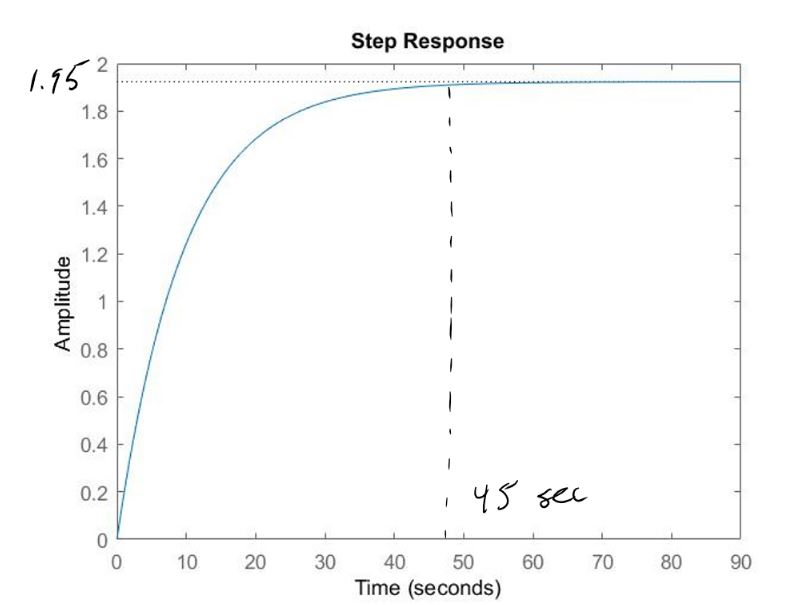
\includegraphics[width=.6\linewidth]{Step(c).JPG}
        \caption{Steady-state and rise-time estimation}
        \label{fig:stepc}
    \end{figure}

    \item[(d)] The final value theorem goes as follow

    \begin{eqnarray}
        \lim_{t\to\infty} f(t) = \lim_{s\to0}s F(s)\\
        \lim_{s\to0}s \frac{1}{s}\frac{0.002}{0.01s + 0.00104} = \frac{0.002}{0.00104} = 1.923
    \end{eqnarray}
    This is 0.27 rad/sec error, or a 14\% overshoot, so my estimate was not that great.
    \item[(e)] As we derived earlier, the transfer function between shaft angle and voltage is $$\frac{\Theta}{V} = \frac{1}{s}\frac{0.002}{0.01s + 0.00104}$$
    \item[(f)] If we add feedback to our system, we get the following block diagram, where $G(s)$ is our plant, in this case, the motor.
    \begin{figure}[!htb]
        \centering
        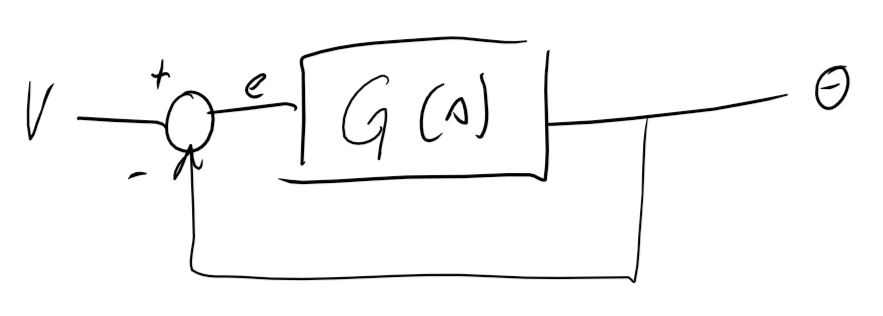
\includegraphics[width=.8\linewidth]{blockf1.JPG}
        \caption{Motor with feedback system}
        \label{fig:f1}
    \end{figure}
    This system can be modeled by the following transfer function:
    $$H(s) = \frac{G(s)}{1+G(s)}$$
    Next we want to add a gain of K to the forward path of the system, this yields the following diagram
    \begin{figure}[!htb]
        \centering
        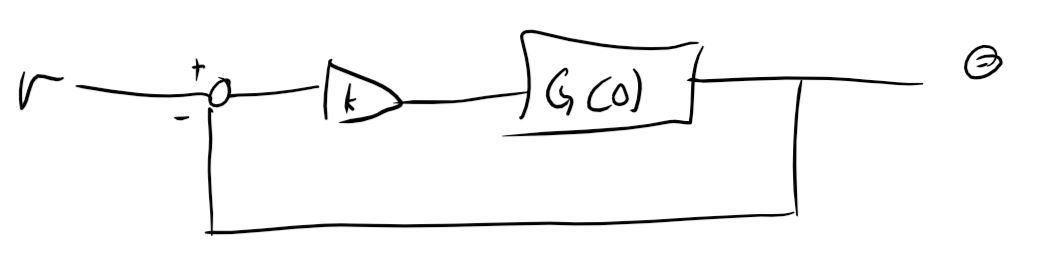
\includegraphics[width=.8\linewidth]{blockf2.JPG}
        \caption{Motor with feedback system and gain on forward path}
        \label{fig:f2}
    \end{figure}
    and is described by the following transfer function:
    $$H(s) = \frac{kG(s)}{1+kG(s)}$$

    \item[(g)] $k$ is gain, unit-less, or V/V
    \item[(h)] From the system diagrams in figure \ref{fig:f2}, we can clearly see the input to the plant $G(s)$ is $k*e(s)$. We can a value for this expression like so. First we find an expression for $e(s)$ and one for $\Theta(s)$:
    \begin{eqnarray}
        e(s) = V(s) - \Theta(s)\\
        \Theta(s) = e(s)*k*G(s)
    \end{eqnarray}
    We isolate $\Theta(s)$ in both expression, equate the equations and isolate $k*e(s)$
    \begin{eqnarray}
        \Theta(s) = V(s) - e(s)\\
        V(s) - e(s) = e(s)*k*G(s)\\
        e(s) \left(k*G(s) + 1\right) = V(s)\\
        e(s) = \frac{V(s)}{k*G(s) + 1}\\
        k*e(s) = \frac{k*V(s)}{k*G(s) + 1}
    \end{eqnarray}

    \item[(i)] Next, we will replace out plant equation in the transfer function of the feedback system $$H(s) = \frac{kG(s)}{1+kG(s)}$$ where $G(s)=\frac{1}{s}\frac{0.002}{0.01s + 0.00104}$
    \begin{eqnarray}
        H(s) &=& \frac{k\left(\frac{0.002}{0.01s^2 + 0.00104s}\right)}{1+k\left(\frac{0.002}{0.01s^2 + 0.00104s}\right)}\\
        H(s) &=& \frac{\frac{k0.002}{0.01s^2 + 0.00104s}}{\frac{0.002k+0.01s^2 + 0.00104s}{0.01s^2 + 0.00104s}}\\
        H(s) &=& \frac{k0.002}{0.01s^2 + 0.00104s}\frac{0.01s^2 + 0.00104s}{0.002k+0.01s^2 + 0.00104s}\\
        H(s) &=& \frac{k0.002}{0.002k+0.01s^2 + 0.00104s}
    \end{eqnarray}
\item[(j)]We can use Matlab and plot this transfer function for different values of $k$ :
\begin{figure}[!htb]
\centering
\begin{subfigure}{.32\textwidth}
  \centering
  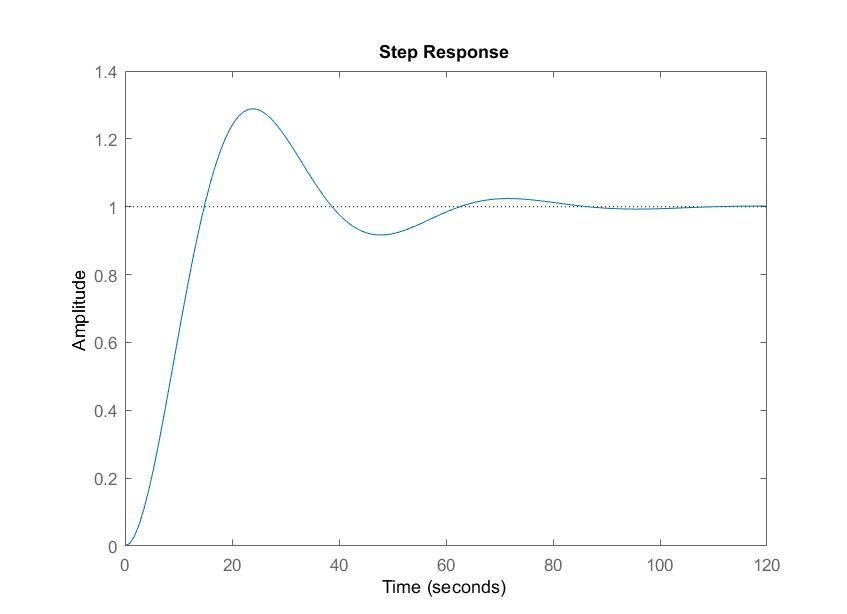
\includegraphics[width=0.9\linewidth]{k1.jpg}
\end{subfigure}
\begin{subfigure}{.32\textwidth}
  \centering
  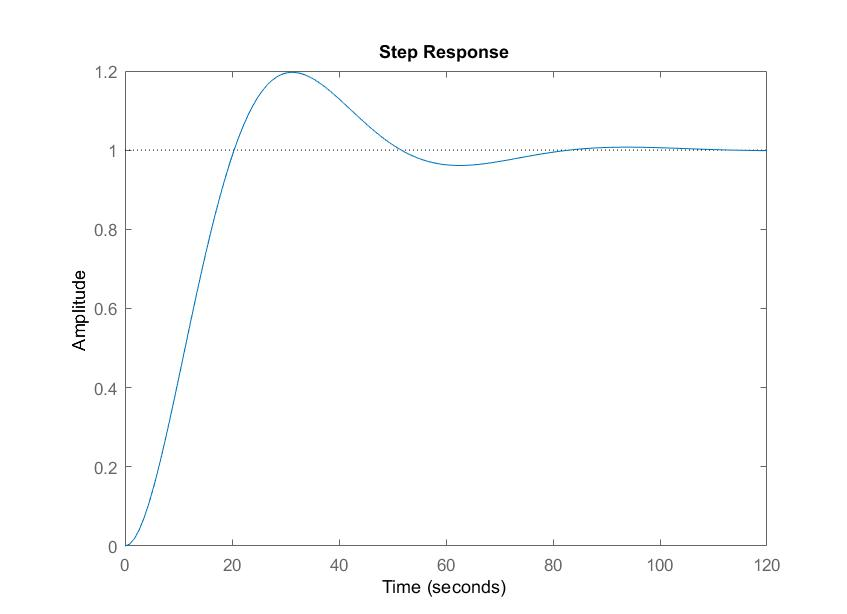
\includegraphics[width=0.9\linewidth]{k064.jpg}
\end{subfigure}
\begin{subfigure}{.32\textwidth}
  \centering
  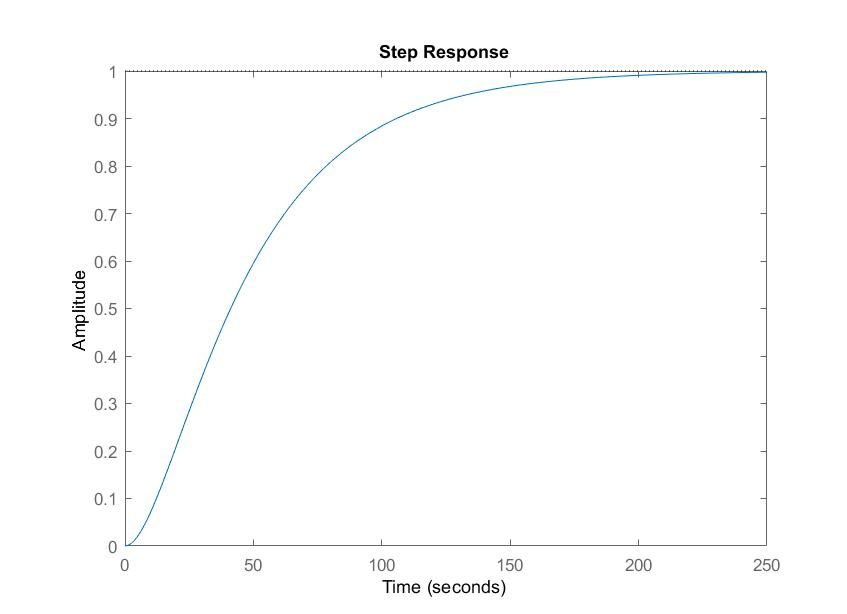
\includegraphics[width=0.9\linewidth]{k01.jpg}
\end{subfigure}
\caption{Servo motor response with different gains}
\end{figure}
We find that a maximum value of 0.064 is acceptable to not overshoot past 20\%.
\clearpage

\item[(k)] In order to reduce our rise-time, we will increase our gain $k$. If we increase it to a value or 1, our rise-time goes down under 4 seconds, and lead to the following step response:
    \begin{figure}[!htb]
        \centering
        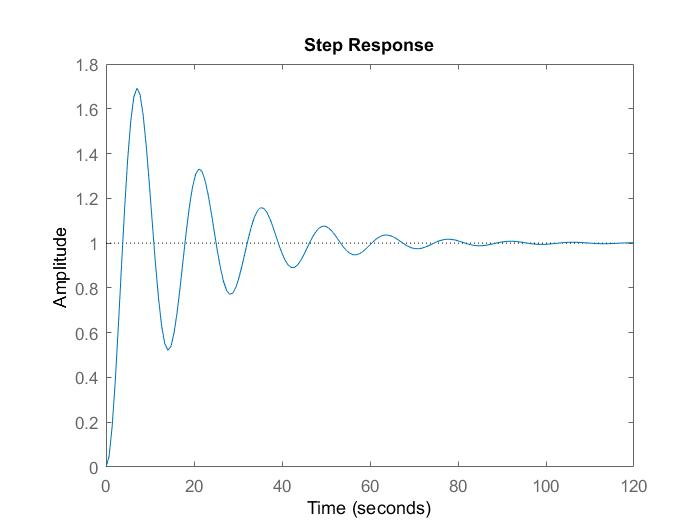
\includegraphics[width=.6\linewidth]{k10.jpg}
        \caption{Motor with feedback system and a gain 10}
    \end{figure}

    \item[(l)] With a value of 0.5 for $k$, we get the following response:
    \begin{figure}[!htb]
        \centering
        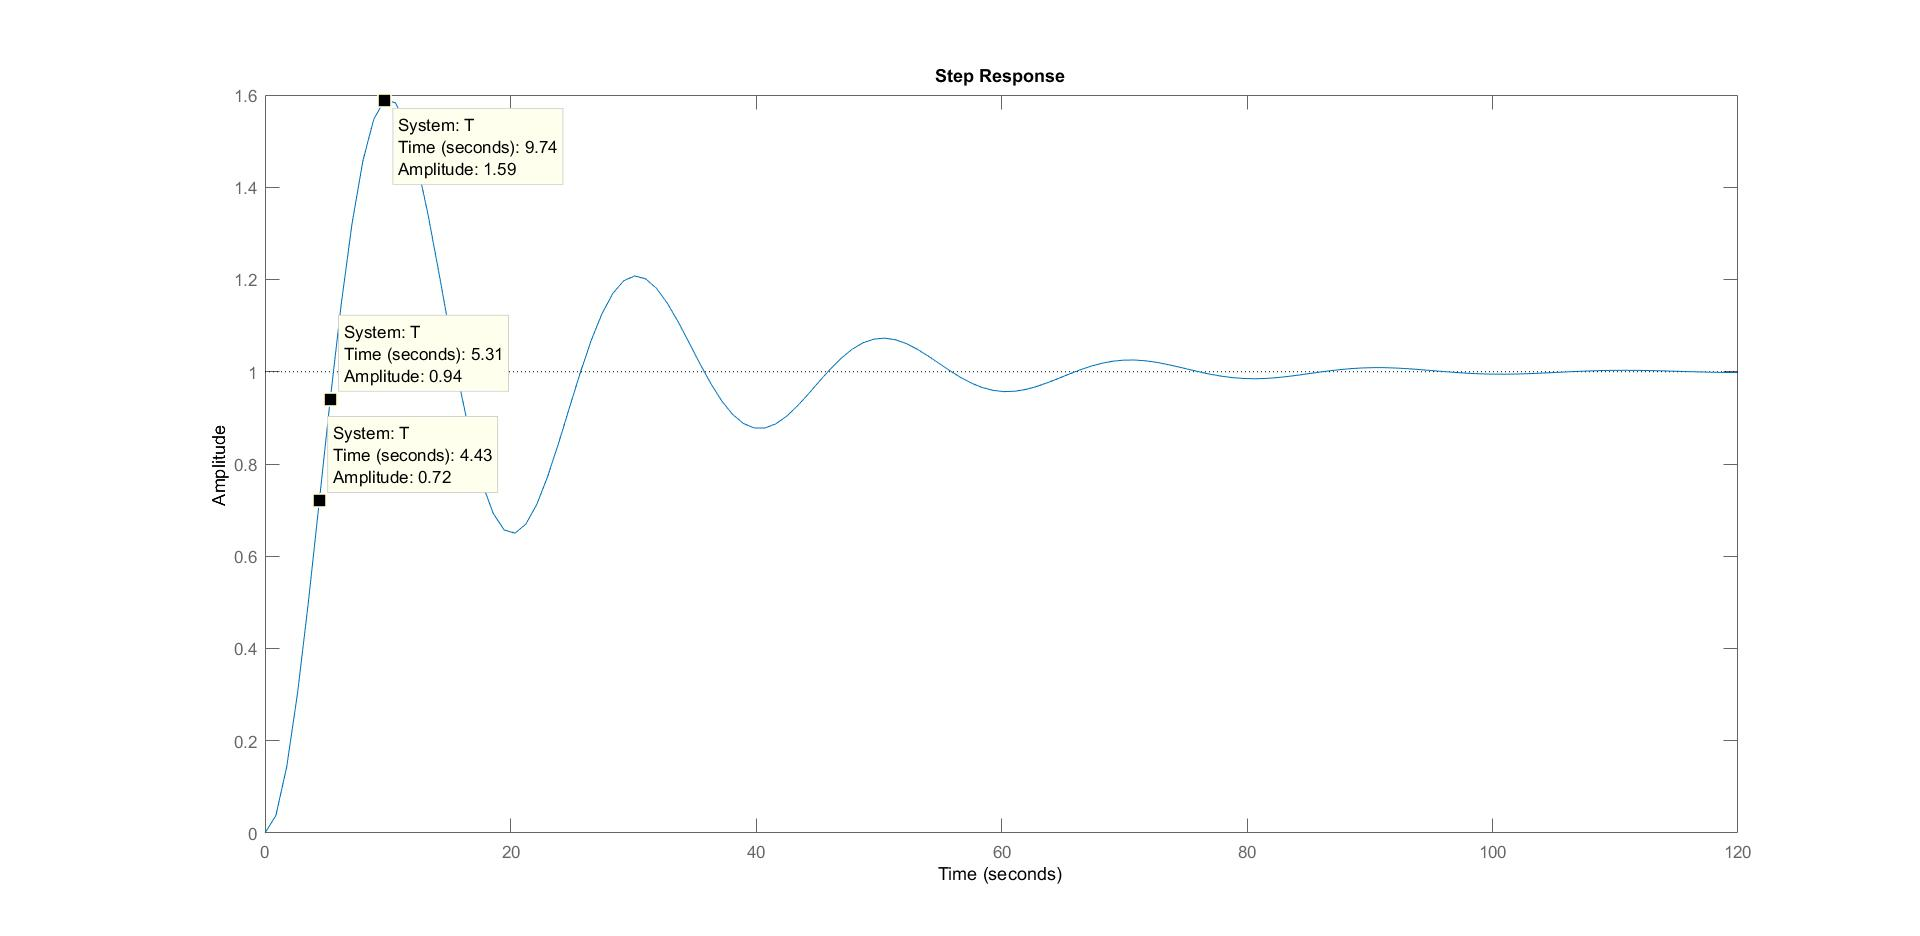
\includegraphics[width=.6\linewidth]{l5.jpg}
    \end{figure}
    For this diagram, we can approximate a rise-time of 4.7 seconds and an overshoot of 59\%.\\
    With a value of 1 for $k$, we get the following response:
    \begin{figure}[!htb]
        \centering
        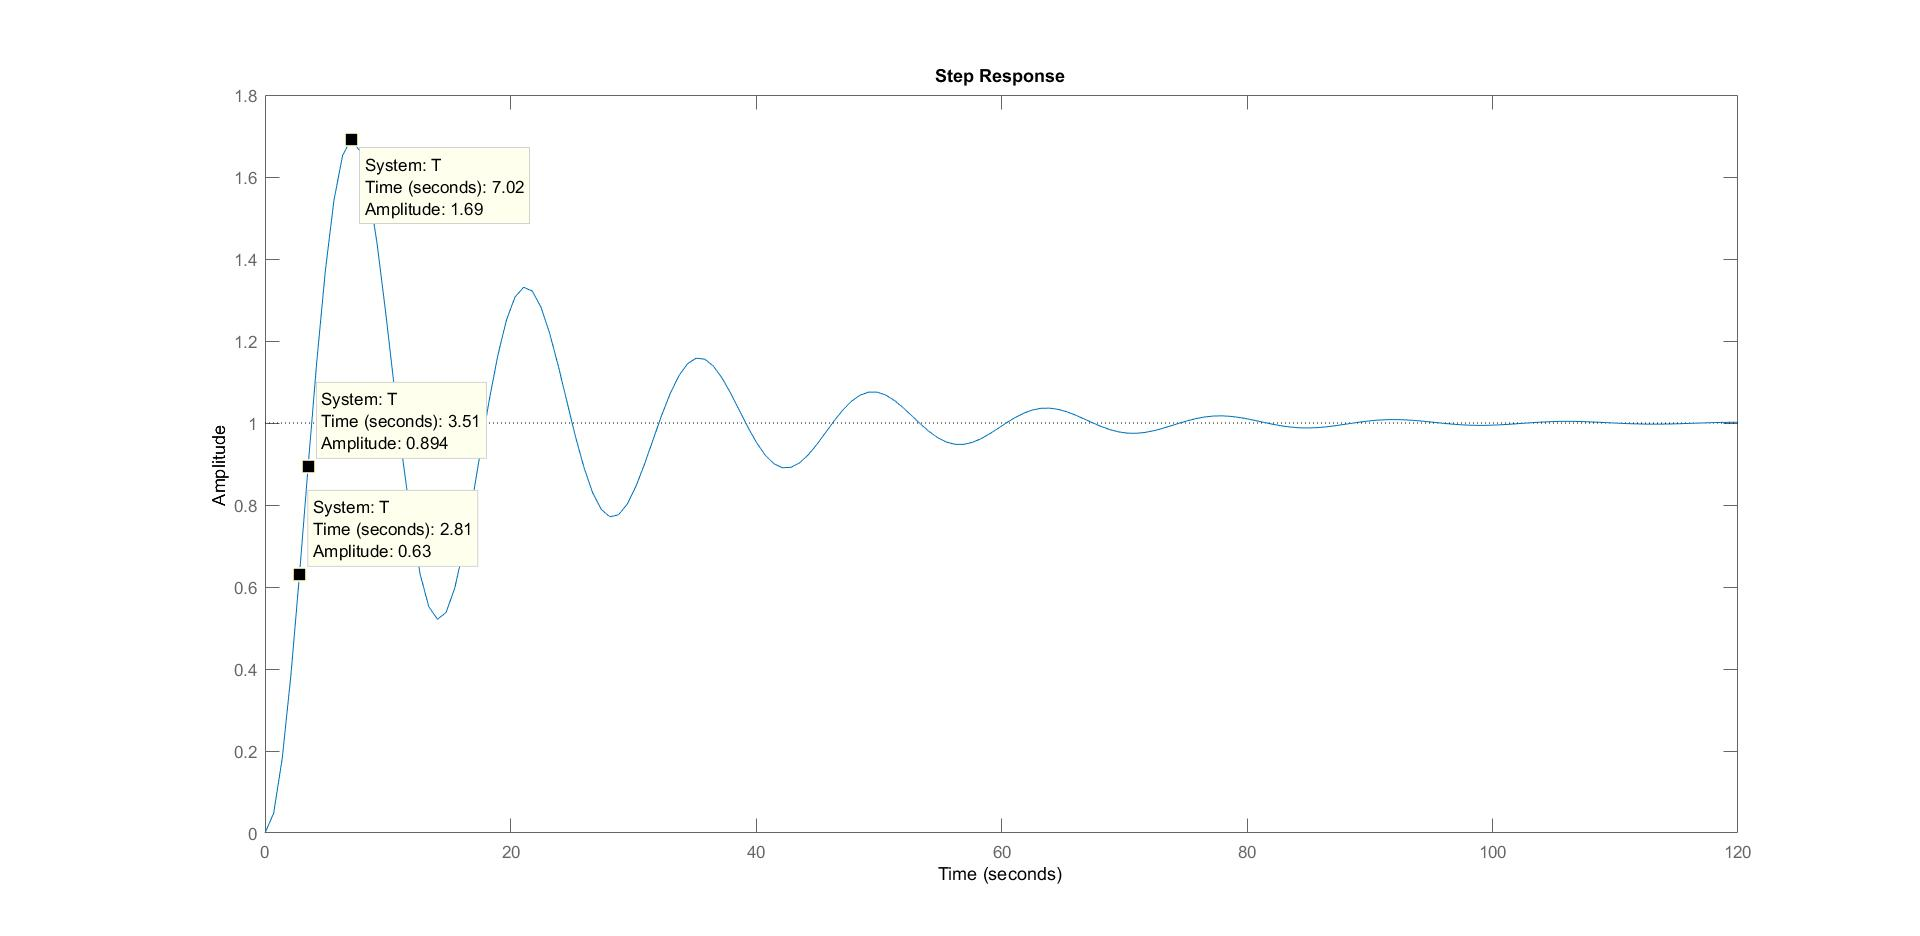
\includegraphics[width=.6\linewidth]{l1.jpg}
    \end{figure}
    For this diagram, we can approximate a rise-time of 3.2 seconds and an overshoot of 69\%.\\
    With a value of 2 for $k$, we get the following response:
    \begin{figure}[!htb]
        \centering
        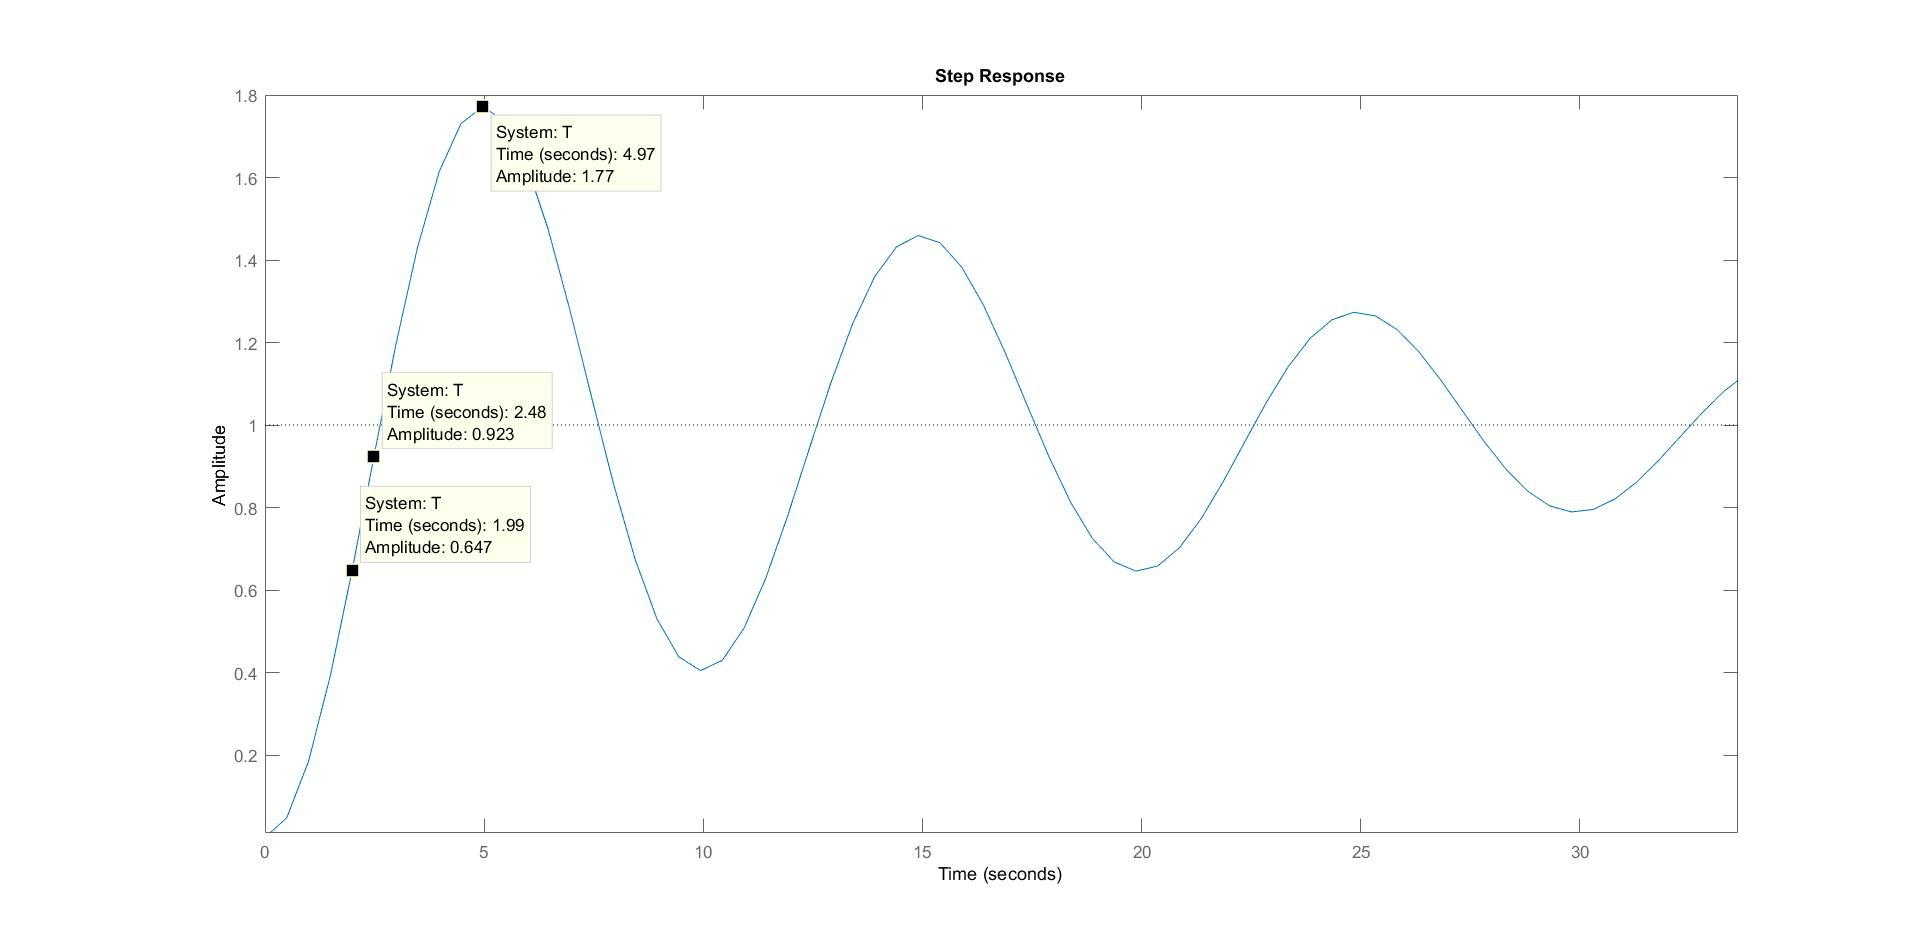
\includegraphics[width=.6\linewidth]{l2.jpg}
    \end{figure}
    For this diagram, we can approximate a rise-time of 2.4 seconds and an overshoot of 77\%.\\
    \item[(m)] With this experiment, we see that the parameter $k$ influences the rise-time of the system, more specifically, how aggressive the corrections are. We can see that a large $k$ value means a very fast acting system, but the system has a high inertia, so it is not able to stop when it approaches it's target. A large gain leads to fast rise-time, large oscillations, and long settling time.
\end{itemize}

\section{}
\begin{itemize}
    \item [(a)] In this code $p$ and $q$ are the coefficients of the numerator and denominator of a transfer function, specifically $$\frac{s+1}{s^3+5s^2+6s}$$
    \item [(b)] The root locus diagram show how the poles of a system will change as some parameters in the transfer function change from $0$ to $\infty$.
\end{itemize}
\end{document}